%% Slides for ".NET Programming" by Chunyu Wang <chunyu@hit.edu.cn> %% -*- coding: utf-8 -*-

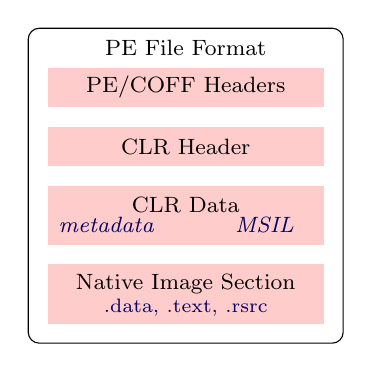
\begin{tikzpicture}[font=\footnotesize]
\draw[rounded corners] (0,.25) rectangle (4,4.25);
\fill[red!20] (.25,.5) rectangle +(3.5,.75);
\fill[red!20] (.25,1.5) rectangle +(3.5,.75);
\fill[red!20] (.25,2.5) rectangle +(3.5,.5);
\fill[red!20] (.25,3.25) rectangle +(3.5,.5);
\node at (2,4) {PE File Format};
\node at (2,3.5) {PE/COFF Headers};
\node at (2,2.75) {CLR Header};
\node at (2,2) {CLR Data};
\node at (1,1.75) {\color{blue!40!black}\textit{metadata}};
\node at (3,1.75) {\color{blue!40!black}\textit{MSIL}};
\node at (2,1) {Native Image Section};
\node at (2,.7) {\color{blue!40!black}\scriptsize .data, .text, .rsrc};
\end{tikzpicture}
